% !TeX program = lualatex
% !TeX encoding = utf8
% !TeX spellcheck = uk_UA
% !TeX root =../LabWork.tex

\keywords{когерентність, інтерференція світла, оптична довжина ходу хвилі, інтерференційна схема}
\abstract{Вивчення явища інтерференції світла; дослідження інтерференційної картини отриманої за допомогою біпризми Френеля; визначення відстані між уявними джерелами в інтерференційному досліді; визначення заломлюючого кута призми; довжини світлової хвилі}
\chapter{Вивчення інтерференції світла за допомогою біпризми Френеля}
\makeworktitle



\section{Теоретичне підґрунтя}

У цій роботі вивчається інтерференційна картина, що отримується \emph{метод поділу хвильового фронту}.

\begin{figure}
	\centering
	\begin{tikzpicture}
		\coordinate (S) at (-5,0);
		\draw[cyan,fill=cyan!50!white](0,0) -- ++(0,2) coordinate (E2) -- ++(0.2,-2) -- +(-0.2,-2) coordinate (E1) -- cycle;
		\draw[red, decoration={
					markings,
					mark=at position 0.5 with {\arrow{latex}}}, postaction={decorate}] (S) -- (E1);
		\draw[red, decoration={
					markings,
					mark=at position 0.5 with {\arrow{latex}}}, postaction={decorate}] (S) -- (E2);
		\draw (10,-4) -- +(0,8) coordinate[pos=0.1] (Ek1) coordinate[pos=0.9] (Ek2) coordinate[pos=0.5] (O);
		\draw[red, decoration={
					markings,
					mark=at position 0.5 with {\arrow{latex}}}, postaction={decorate}] (E1) -- (Ek1);
		\draw[red, decoration={
					markings,
					mark=at position 0.5 with {\arrow{latex}}}, postaction={decorate}] (E2) -- (Ek2);
		\draw[dash dot] (S) -- (O);
		\draw[dashed] let \p{E1Ek1} = ($(Ek1) - (E1)$) in (E1) -- (-5,{-2cm-5cm*\y{E1Ek1}/\x{E1Ek1}}) coordinate (S1);
		\draw[dashed] let \p{E2Ek2} = ($(Ek2) - (E2)$) in (E2) -- (-5,{2cm-5cm*\y{E2Ek2}/\x{E2Ek2}}) coordinate (S2);
		\draw[dashed] (S1) -- (0,0); \draw[red!50, decoration={
					markings,
					mark=at position 0.5 with {\arrow{latex}}}, postaction={decorate}] let\p{S1E} = ($(S1) -  (0,0)$) in (0,0) -- (10,{10cm*\y{S1E}/\x{S1E}}) coordinate (EkS1);
		\draw[dashed] (S2) -- (0,0); \draw[red!50, decoration={
					markings,
					mark=at position 0.5 with {\arrow{latex}}}, postaction={decorate}] let \p{S2E} = ($(S2) -  (0,0)$) in (0,0) -- (10,{10cm*\y{S2E}/\x{S2E}}) coordinate (EkS2);
		\draw[decorate,decoration={brace,amplitude=5pt,raise=1ex}] (S1) -- node[left=2ex] {$d$} (S2);

		\draw (S1) -- ([yshift=-2.1cm]S1);
		\draw[latex-latex] ([yshift=-2cm]S1) -- node[fill=white] {$a$} +(5,0) coordinate (R);
		\draw[latex-latex] (R) -- node[fill=white] {$b$} +(10,0);
		\draw (0,-2) -- ([yshift=-0.1cm]R);

		\begin{scope}[on background layer]
			\fill[red!10] (0,0) -- (EkS1) -- (EkS2);
 		\end{scope}

		\draw[very thin, red, fill=red] (S) circle(0.05) node[black, above] {$S$};
		\draw[very thin, red, fill=red] (S1) circle(0.05) node[black, above] {$S_1$};
		\draw[very thin, red, fill=red] (S2) circle(0.05) node[black,  above] {$S_2$};
		\foreach \i in {-2.5,-2,...,2.5} { \path[bottom color=white,  top color=white, middle color = red!90!black] (10.1,{\i-0.125}) rectangle +(0.5,0.25); }
	\end{tikzpicture}
	\caption{Схема інтерференції на біпризмі}
	\label{fig:biprismscheme}
\end{figure}

\begin{wrapfigure}[12]{O}{0.3\columnwidth}
	\centering
	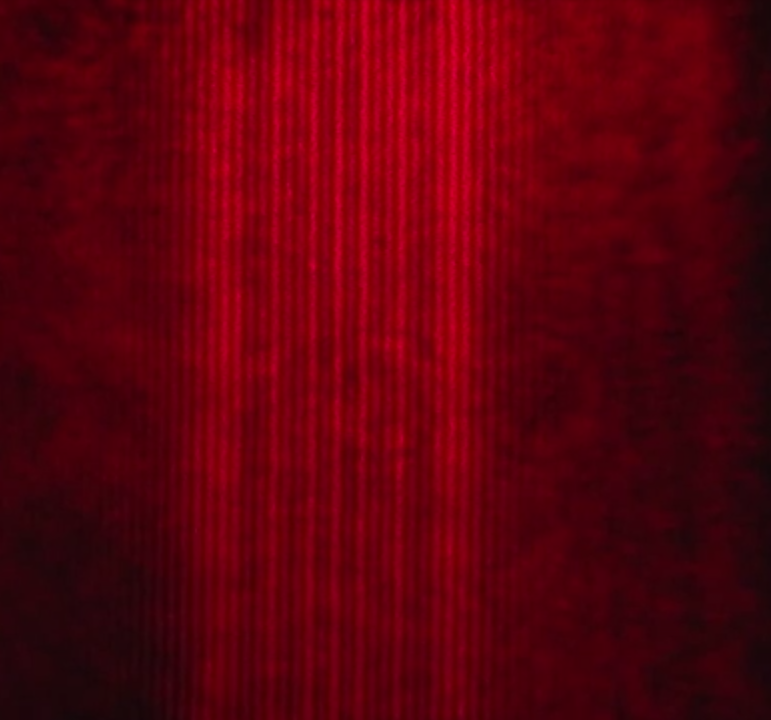
\includegraphics[width=\linewidth]{\currfiledir/biprism_map}
	\caption{Інтерференційна картина}
	\label{fig:biprism_map}
\end{wrapfigure}
Для отримання інтерференції джерело світла $S$ розташовують симетрично відносно призм, що створюють біпризму. Кути падіння променів на поверхні призми малі, тому всі промені, що відхиляються нею на однаковий кут
\begin{equation}
	\varphi = (n-1)\beta,
\end{equation}
де $n$ -- показник заломлення матеріалу, з якого виготовлена призма, а $\beta$ -- заломлюючий кут призми (див. рис.~\ref{fig:biprismscheme}).

В результаті такого заломлення утворюються два когерентних пучка світла, вершини яких $S_1$ і $S_2$ можна розглядати, як точки розташування уявних зображень джерела $S$. На екрані когерентні промені від джерел $S_1$ і $S_2$ перекриваються і формують інтерференційну картину, що являє собою набір світлих і темних смуг, що чергуються (рис.~\ref{fig:biprism_map}).

В експериментах з біпризмою Френеля інтерференційні смуги спостерігаються в області перекриття пучків на екрані при будь-якій відстані від екрана до біпризми. Про такі смуги кажуть, що вони не локалізовані.

\subsection{Схема досліду та робочі формули}

З рис.~\ref{fig:YoungScheme} видно, що
\begin{equation}
	\frac{d}{2} = a \tg\phi  \cong a(n-1)\beta.
\end{equation}
Звідки
\begin{equation*}
	d  = 2a(n-1)\beta.
\end{equation*}
Використавши формулу для ширини інтерференційного максимуму з \eqref{eq:widthofmax} отримаємо.
\begin{equation}
	\Delta y = \frac{L \lambda }{2a (n - 1)\beta} \label{eq:deltax}.
\end{equation}


Отже, вимірюючи відстань між інтерференційними смугами $\Delta y$, відстань від фокуса лінзи до біпризми $a$ та відстань від лінзи до інтерференційної картини $L$, можна визначити одну з трьох величин $\lambda$, $\beta$, або $n$, якщо відомі дві інші.

\section{Опис робочої установки}

\begin{figure}[h!]
	\centering
	\begin{tikzpicture}[scale=2, every pic/.style={scale=2}, xscale=-1]
		%    	\draw (-5,-5) to [grid with coordinates] (5,5);
		\pic at (0,0) {lava};
		\pic at (2,0.1)  {reuter};
%		\pic (l) at (2,1.8) {lens};
%		\pic (L) at (3,1.8)  {laser};
%		\draw[] (L-top) -- ++(45:1) node[above] {$1$};
%		\pic at (0,0.1) {reuter};
%		\pic (P) at (0.05,1.8) {biprism};
%		\draw[] (l-lens) -- ++(-135:1) node[below] {$2$};
%		\draw[] (P-top) -- ++(45:1) node[above] {$3$};
%		\pic at (-3,0.1) {reuter};
%		\pic (E2) at (-3,1.8) {ecran};
%		\draw[] (E2-top) -- ++(45:1) node[above] {$4$};
%		\draw[dash dot] (-4,1.8) -- (4,1.8);
	\end{tikzpicture}
	\caption{Робоча установка}
	\label{fig:biprism_scheme}
\end{figure}
Промені лазера \hyperref[fig:biprism_scheme]{$1$} направляються на збиральну лінзу \hyperref[fig:biprism_scheme]{$2$}, фокусуються на її оптичній осі, а потім потрапляють на біпризму Френеля \hyperref[fig:biprism_scheme]{$3$}. Фокус збиральної
лінзи є моделлю точкового джерела когерентного монохроматичного світла. При такій оптичній схемі збільшується яскравість інтерференційних смуг. Для спостереження інтерференційних смуг використовується, або телескопічна система з мікрометричним окуляром, або екран \hyperref[fig:biprism_scheme]{$4$} (в якості екрана можна вибрати стінку лабораторії).



Використання телескопічної системи в лабораторній роботі, вимагає деякого уточнення формули \eqref{eq:deltax}.


\section{Хід роботи}

\begin{enumerate}
	\item Зберіть установку відповідно до рис.~\ref{fig:biprism_scheme}. Біпризму розташуйте на відстані не меншою ніж $10$~см від лінзи.
	\item Визначте відстань від лінзи до біпризми $a$.
	\item Визначте відстань від біпризми до екрану, на якому спостерігається інтерференційна картина $b$.
	\item  Визначте кутову відстань між інтерференційними смугами $\tg\phi = \frac{\Delta x}{b}$.

	      Досліди проведіть для $10$ відстаней.

	\item  За формулою \eqref{eq:deltax} розрахуйте для кожного досліду заломлюючий кут біпризми.
	      Френеля.
\end{enumerate}

\section*{Контрольні запитання}
\addcontentsline{toc}{section}{Контрольні запитання}
\begin{enumerate}[label*=\arabic*.]
    \item Виведіть формули визначають положення інтерференційних максимумів і ширину
    смуги (періоду інтерференційної картини) для оптичної схеми з двома точковими
    джерелами світла.
    \item Чому інтерференційна картина може спостерігатися лише при малій відстані між когерентними джерелами? Що таке радіус когерентності?
    \item  Оцініть максимальне число інтерференційних смуг, яке можна спостерігати в умовах досвіду.
\end{enumerate}
